\documentclass{article}
\usepackage{amsthm}
\usepackage{amsmath}
\usepackage{etoc}
\usepackage{amssymb}
\usepackage{enumitem}
\usepackage{apacite}
\usepackage{mathtools, amssymb}
\usepackage{bm}
\usepackage{tikz}
\usepackage{fancyhdr}
\usepackage{caption}
\usepackage{tabto}
\usepackage{hyperref}
\usepackage{graphicx}
\usepackage[nottoc]{tocbibind}
\usepackage{calrsfs}
\usepackage{changepage}
\usepackage{siunitx}
\usetikzlibrary{arrows.meta, automata, positioning, quotes}



% Margins
\usepackage[top=2.5cm, left=3cm, right=3cm, bottom=4.0cm]{geometry}
% Colour table cells

% Get larger line spacing in table
\newcommand{\tablespace}{\\[1.25mm]}
\newcommand\Tstrut{\rule{0pt}{2.6ex}}         % = `top' strut
\newcommand\tstrut{\rule{0pt}{2.0ex}}         % = `top' strut
\newcommand\Bstrut{\rule[-0.9ex]{0pt}{0pt}}   % = `bottom' strut

%%%%%%%%%%%%%%%%%
%     Title     %
%%%%%%%%%%%%%%%%%
\title{Theory of automata and Formal languages}
\author{Fernando Javier López Cerezo \\ Practice 2}
\date{\today}

\begin{document}
\maketitle

%%%%%%%%%%%%%%%%%
%   Problem 1   %
%%%%%%%%%%%%%%%%%
In practice 2 we are asked to build a DFA over the alphabet $\{a,b\}$ that contains only the string a. This is my proposed solution:
\section*{Part 1}
We start by writing the DFA in a style similar to the one in talflecturenotes: \\\\ Let $M=(\{q_0,q_1,q_2\}, \{a,b\}, \delta, q_0, \{q_1\})$ be a DFA with:\\

\begin{table}[h!]
\begin{tabular}{c|c|c}
  $\delta(q,\sigma)$ & $a$ & $b$\\
  \hline
  $q_0$& $q_1$ & $q_2$\\
  \hline
  $q_1$& $q_2$ & $q_2$\\
  \hline
  $q_2$& $q_2$ & $q_2$
\end{tabular}
\end{table}

\begin{center}
  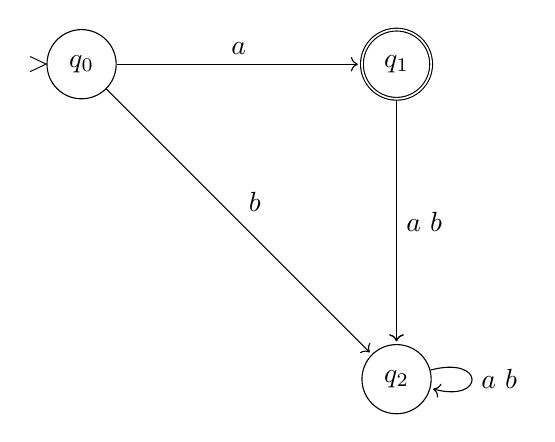
\begin{tikzpicture}[auto,
      shorten > = 1pt, 
  node distance = 4cm and 3cm]
  \node[state] (q0) {$q_0$};
  \node[inner sep=0pt,outer sep=-1pt,left=0pt of q0.west]{$>$};
  \node[state, accepting] (q1) [right of=q0] {$q_1$};
  \node[state] (q2) [below of=q1] {$q_2$};
  \path[->] (q0) edge ["$a$"] (q1)
                 edge ["$b$"] (q2)
            (q1) edge ["$a \text{ } b$"] (q2)
                 edge ["$ $"] (q2)
            (q2) edge [loop right, "$a \text{ } b$"] ();
  \end{tikzpicture}
\end{center}
\newpage
\section*{Part 2}
Now we create the same DFA using JFLAP: \\\\
\includegraphics[width=\linewidth]{DFA.png} \\\\ If we test it with 6 random strings we can check that it works: \\\\ \includegraphics[width=\linewidth]{table.png}
\newpage
\section*{Part 3}
Finally we express the DFA in a JSON file : \\\\ 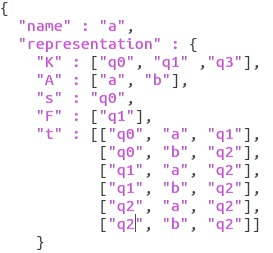
\includegraphics[width=\linewidth]{automata.png} \\\\ We use Octave to test it with a few strings: \\\\ 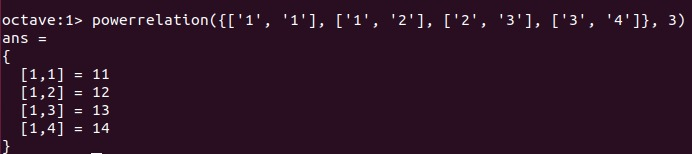
\includegraphics[width=\linewidth]{octave.png} \\ 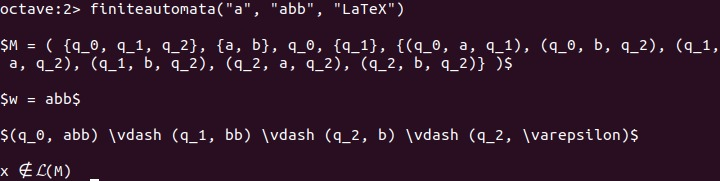
\includegraphics[width=\linewidth]{octave2.png} \\\\ 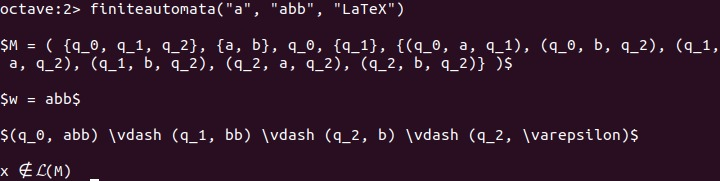
\includegraphics[width=\linewidth]{octave2.png}


\end{document}